\section{Metodologia}
\label{sec:metodologia}

In questa sezione verranno descritti in dettaglio l'approccio usato per il lavoro di gruppo e le funzioni di reperimento realizzate.


\subsection{Approccio}
\label{sec:approccio}

L'obiettivo delle funzioni di reperimento implementate \'e di massimizzare la Mean Average Precision (\textsc{MAP}). Per calcolarla e verificarne il cambiamento durante le varie versioni del codice viene utilizzato \texttt{trec\_eval}, esso e' il tool standard usato dalla TREC community per valutare l'efficacia del reperimento. Tale strumento prende in input un file di risultati del reperimento, e un file con i giudizi di rilevanza \textit{qrels-treceval.txt}, e fornisce un insieme di misure di efficacia.

E' stato scelto di utilizzare un metodo probabilistico per la risoluzione dei laboratori. In particolare e' stato utilizzato l'algoritmo \textsc{bm25} \cite{melucci2013information} poiche' \'e un buon modello, ed \'e stato usato con successo in letteratura \cite{croft2010search}.  Per realizzare le implementazioni e' stato utilizzato Python, corredato da diverse librerie: \texttt{numpy/scipy} per la gestione delle matrici, \texttt{matplotlib} per il plot dei risultati, \texttt{networkx} per la gestione dei grafi.
Per il versionamento si e' scelto \texttt{Git}. Tutto il codice prodotto e' disponibile online \cite{repoonline}. 

Per lo svolgimento dei laboratori \'e stato utilizzato un approccio di gruppo. Durante le ore di laboratorio i componenti del gruppo affrontavano una discussione, riguardante sia gli aspetti teorici che pratici trattati. Veniva quindi deciso come procedere, e durante un successivo incontro venivano definiti i dettagli del lavoro svolto e venivano prodotti i documenti da consegnare.

\subsection{Indicizzazione} \label{sec:metodi-di-indic}

\paragraph{\textbf{Descrizione.}} 
Costruzione di un algoritmo di indicizzazione in grado di costruire delle strutture dati necessarie al reperimento con \textsc{bm25}. 

\paragraph{\textbf{Implementazione.}}
Per l'implementazione e' stato utilizzato il file \textit{freq.docid.stem.txt} che contiene le frequenze delle keywords (dopo lo stemming) nei documenti. Poiche' le stop words sono gia' state rimosse da tale file, viene ignorata la stoplist. L'algoritmo di indicizzazione utilizza le keywords presenti in tale file per costruire un dizionario delle keywords presenti nella collezione. In seguito scorre sulle righe del file \textit{freq.docid.stem.txt} e costruisce la Document Term Matrix (DTM), una matrice di  dimensione $n_{docs} \times n_{words}$ che contiene in posizione $(j,i)$ il numero di occorrenze del termine $j$ nel documento $i$. Infine salva su file le seguenti strutture:
\begin{itemize}
	\item Le lunghezze (numero di termini) dei documenti, necessarie alla normalizzazione sulla lunghezza in \textsc{bm25},
	\item La matrice DTM,
	\item La DTM normalizzata sulle colonne, cioe' una matrice delle frequenze che contiene in posizione $(j,i)$ la frequenza del termine $i$ nel documento $j$, nel resto del documento verra' fatto riferimento a questa matrice come FDTM,
	\item Il dizionario contenente le keywords della collezione.
\end{itemize}

\subsection{Reperimento}
\label{sec:metodi-di-reper}

\paragraph{\textbf{Descrizione}}
Comprensione dei meccanismi di reperimento e costruzione di un primo algoritmo di reperimento.
Realizzazione dell'algoritmo \textsc{bm25}, che riceve in input una query e restituisce una lista ordinata di documenti con i relativi punteggi. Per chiarezza viene riportata la formula del reperimento tramite tale algoritmo (per il documento $j$), si rimanda al libro \cite{melucci2013information} per la spiegazione completa:
\[ S^{(BM25)}_j = \sum\limits_{i \in Q}\log\Bigl(\frac{N-n_i+0.5}{n_i+0.5}\Bigl)\cdot\frac{(k_1+1)f_i}{k+f_i}\cdot\frac{(k_2+1)qf_i}{k_2+qf_i}. \]


\paragraph{\textbf{Implementazione}}
L'algoritmo scorre la lista dei documenti, e per ognuno di essi calcola e somma il punteggio di \textsc{bm25} per ogni termine della query $qw \in Q$. Le strutture ottenute dall'indicizzazione (Sezione \ref{sec:metodi-di-indic}) vengono utilizzate per tale calcolo. Il dizionario e la matrice FDTM vengono utilizzati per recuperare le frequenze dei termini, mentre le lunghezze dei documenti vengono direttamente inserite nella formula di \textsc{bm25}. Lo pseudocodice per l'algoritmo e' il seguente:
\begin{algorithmic}
\State $C \gets documents$
\State $Q \gets query$
\State $S \gets list()$
\ForAll{$doc \in C$}
	% \State $index\_of\_words \gets extract(D,qw)$
	\ForAll{$qw \in Q$}
		\State $S^{(BM25)}_{doc} = S^{(BM25)}_{doc} + BM25(qw)$
	\EndFor
\EndFor
\State $sort(S)$\\
\Return top $k$ scoring documents
\end{algorithmic}
Tale algoritmo ha complessita' $O(n \cdot m)$, dove $n$ \'e il numero di documenti nella collezione ed $m$ \'e il numero di termini presenti nella query $Q$. Il risultato della funzione di reperimento qui presentata verra' indicato nel resto del documento come \textsc{baseline}. Ai fini dell'efficienza, i due cicli dell'algoritmo sono stati in un secondo momento convertiti in una serie di operazioni su matrici. Grazie ai benefici della $vectorization$ in \texttt{numpy}, cio' ha garantito un notevole miglioramento del tempo di esecuzione.
\subsection{Relevance Feedback}
\label{sec:relevance-feedback}

\paragraph{\textbf{Descrizione}}
Implementazione di una funzione di reperimento che utilizza Relevance Feedback (\textsc{rf}), sia \textsc{esplicito} che \textsc{pseudo}. Nel primo caso, si ricorda che l'algoritmo \textsc{bm25} nella sua forma completa, integra le informazioni di rilevanza:
\[ S^{(RF)}_j = \sum\limits_{i \in Q}\log\Bigl(\frac{(r_i+0.5)/(R-r_i+0.5)}{(n_i-r_i+0.5)/(N-n_i-R+r_i+0.5)}\Bigl)\cdot\frac{(k_1+1)f_i}{k+f_i}\cdot\frac{(k_2+1)qf_i}{k_2+qf_i}, \]
dove $R$ e' il numero di documenti rilevanti per la query considerata, mentre $r_i$ e' il numero di documenti rilevanti che contengono il termine $i$. Mentre nel caso del \textsc{rf esplicito} tali informazioni sono note, nel caso di \textsc{rf pseudo} esse vengono ricavate dopo un primo reperimento con la funzione \textsc{baseline}, dove i primi $N$ documenti sono considerati rilevanti.

\paragraph{\textbf{Implementazione}} 
L'implementazione delle due tipologie di \textsc{rf} \'e differente, poiche' il calcolo dello \textsc{pseudo} richiede due passi, mentre ne basta uno solo per l'\textsc{esplicito}.
\begin{itemize}
\item \textsc{esplicito}: viene utilizzato il file \textit{qrels-treceval.txt}, contenente i giudizi di rilevanza, per estrarre i valori di $R$ ed $r_i$.
\item \textsc{pseudo}: viene eseguito un reperimento con la funzione \textsc{baseline}. Vengono poi considerati rilevanti i primi $N$ documenti reperiti, cioe' $R=N$. Per il calcolo di $r_i$ viene utilizzata FDTM, dove un elemento $FDTM(j, k)>0$ significa che il documento $j$ contiene il termine $k$.
\end{itemize}
I valori di $R, r_i$ vengono inseriti nella formula di \textsc{bm25} per ottenere il ranking finale.

\subsection{PageRank}
\label{sec:pagerank}

\paragraph{\textbf{Descrizione}}
Comprensione di \textsc{pagerank} e implementazione di una funzione di reperimento che lo integri.
E' stata scelta la seguente formula per il ranking. Per ogni documento $j$, essa combina gli score di \textsc{bm25} ($S^{(BM25)}_j$)  con il valore del \textsc{pagerank} ($pr_j$) nel seguente modo:
\[ S^{(PR)}_j =  \alpha \cdot S^{(BM25)}_j + (1-\alpha) \cdot pr_j,\]
dove $\alpha$ e' un parametro che varia tra 0 ed 1 e, quindi, sposta il peso uniformemente da \textsc{pagerank} a \textsc{bm25}.
Per poter effettuare tale somma in modo coerente, entrambe le distribuzioni (gli score di \textsc{bm25} e i valori di \textsc{pagerank}) devono essere scalate. E' stato scelto di normalizzare gli $S^{(BM25)}_j$ e i $pr_j$ in modo da avere valori compresi tra 0 e 1. Per far ci\'o abbiamo usato la formula:
\[ z_i = \frac{x_i - min(x)}{max(x) - min(x)}, \]

\paragraph{\textbf{Implementazione}}
Per effettuare il calcolo del \textsc{pagerank} abbiamo utilizzato la libreria \texttt{networkx}, essa attraverso il metodo \texttt{read\_edgelist} permette la costruzione del grafo delle citazioni a partire da una lista di archi, contenuta nel file \textit{citazioni.txt}. Inoltre dispone del metodo \texttt{pagerank} per la computazione del \textsc{pagerank} utilizzando \textsc{power iteration} sulla matrice di transizione. Tale computazione e' fatta a tempo di indicizzazione, e i valori sono salvati su un file. A tempo di reperimento l'algoritmo effettua il reperimento con la funzione \textsc{baseline} e poi combina i risultati usando i valori di \textsc{pagerank} per calcolare il punteggio finale. La normalizzazione viene effettuata con metodi e operazioni su vettori.

\subsection{Latent Semantic Analysis}
\label{sec:lsa}

\paragraph{\textbf{Descrizione}}
Comprensione di Latent Semantic Analysis (\textsc{lsa}) e costruzione di una funzione di reperimento che integri \textsc{lsa}. E' stato scelto di utilizzare \textsc{lsa} per riordinare i primi $N$ documenti reperiti con la funzione di reperimento \textsc{baseline}. 

\paragraph{\textbf{Implementazione}} 
L'algoritmo effettua il reperimento con la funzione \textsc{baseline}, e prende in considerazione soltanto i primi $N$ documenti reperiti. Filtra quindi la matrice DTM in maniera che le uniche righe considerate siano quelle relative agli $N$ documenti considerati, e successivamente rimuove i termini (le colonne) che non compaiono in tale matrice. Ci riferiamo alla matrice cosi' ottenuta come $X$, che rappresenta ora il nostro spazio delle feature. Viene poi utilizzato il metodo \texttt{numpy.linalg.svd} per il calcolo della fattorizzazione della matrice $X$: 
\[ X = U \Sigma V^{T}. \]
Vengono poi considerate $m$ dimensioni, ottenendo quindi la matrice ridotta: 
\[ X_m = U_m \Sigma_m V^{T}_m. \]
Viene poi effettuata la proiezione del vettore query $\vec{q}$ sullo spazio a dimensione ridotta secondo la formula: 
\[ \vec{q}_m = \Sigma^{-1}_m U^{T}_m \vec{q}. \]
Infine l'algoritmo calcola la \textit{cosine similarity} tra le rappresentazioni degli $N$ documenti nello spazio ridotto (cioe' le colonne $V^{T}_m$) e la query ridotta $\vec{q}_m$. Il ranking per gli $N$ documenti viene modificato rispetto alla similarita' decrescente cosi calcolata. I restanti documenti vengono semplicemente accodati.

\subsection{Hyper-linked Induced Topic Search}
\label{sec:hits}

\paragraph{\textbf{Descrizione}}
Comprensione di Hyperlinked Induced Topic Search (\textsc{hits}), implementazione di una funzione di reperimento che integri \textsc{hits}. E' stato scelto di riordinare i primi $N$ documenti reperiti con la funzione di reperimento \textsc{baseline}. A tal fine viene costruito il grafo radice $G_R$ contente gli $N$ documenti individuati, ed esso viene espanso secondo la dinamica standard: ogni nodo citato dai nodi di $G_R$ o citante i nodi di $G_R$ viene aggiunto al grafo radice di partenza. Il grafo risultante e' detto grafo base $G_B$. Infine per ogni documento $j$ di $G_B$, viene calcolato lo score $S^{(HITS)}_{j}$ con la seguente formula:
\[ S^{(HITS)}_j =  \alpha \cdot S^{(BM25)}_j + \beta \cdot auth_j + \gamma \cdot hub_j,\]
dove $auth_j$ e $hub_j$ indicano rispettivamente il punteggio di autorevolezza e di hubbines per il documento $j$ nel grafo $G_B$. Il valore dei parametri $\alpha, \beta, \gamma$ puo' variare tra [0, 1]. Infine gli $N$ documenti inizialmente individuati vengono riordinati in base al punteggio cosi' ottenuto. Una normalizzazione come quella presentata in Sezione \ref{sec:pagerank} viene utilizzata per ottenere dei punteggi confrontabili per le tre distribuzioni (autorevolezza, hubbiness, punteggio di \textsc{bm25}).
\paragraph{\textbf{Implementazione}}
L'algoritmo effettua il reperimento con la funzione \textsc{baseline}, e prende in considerazione soltanto i primi $N$ documenti reperiti. Carica poi l'intero grafo delle citazioni, caricando la lista di archi contenuta in \textit{citazioni.txt}. Poi viene salvata la lista dei nodi che costituisce il grafo radice $G_R$, e viene effettutata l'espansione iterando sugli archi di tali nodi, ottenendo cosi' una lista di nodi che costituisce i nodi che costituiranno $G_B$. Utilizzando tale lista viene costruito il grafo base. Su tale grafo viene computato \textsc{hits} con il metodo \texttt{networkx.hits}. Le distribuzioni dei punteggi vengono scalate, e infine viene calcolato il $S^{(HITS)}_j$. Infine l'algoritmo modifica il ranking per gli $N$ documenti rispetto al punteggio calcolato. I restanti documenti vengono semplicemente accodati. Figura \ref{fig:hitsexpansion} mostra il grafo radice e il grafo base per la query $56$.

\begin{figure}
	\centering
	\begin{subfigure}{.5\textwidth}
		\centering
		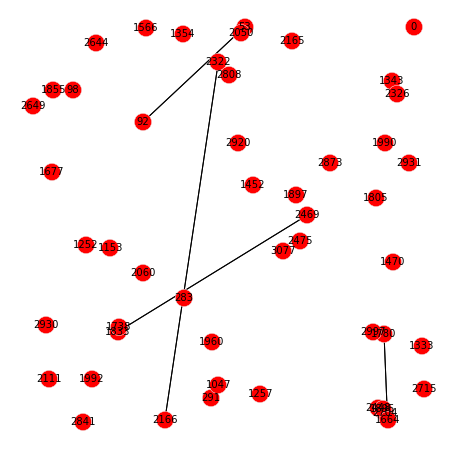
\includegraphics[width=1\textwidth]{figures/R.png}
		\caption{Grafo radice $G_R^{(56)}$}
		\label{fig:uno}
	\end{subfigure}%
	\begin{subfigure}{.5\textwidth}
		\centering
		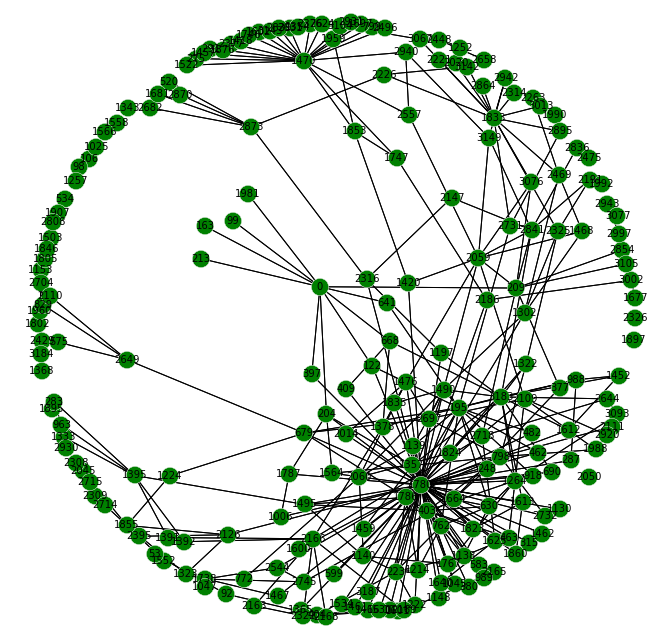
\includegraphics[width=1\textwidth]{figures/B.png}
		\caption{Grafo base $G_B^{(56)}$.}
		\label{fig:due}
	\end{subfigure}
	\caption{Grafi costruiti a partire dai primi $N=50$ documenti reperiti per la query $56$.}
	\label{fig:hitsexpansion}
\end{figure}

\subsection{Evolution Strategy}
\label{sec:es}

Per ottimizzare gli algoritmi di reperimento abbiamo scelto di utilizzare un Evolution Strategy~\cite{back1996evolutionary} (ES), una tecnica di ottimizzazione basata sui principi che regolano l'evoluzione. Tecniche di questo tipo sono piu' robuste rispetto ai metodi di ricerca lineare per quanto riguarda i massimi locali. Il loro svantaggio consiste nel maggior numero di valutazioni richieste. Nel nostro contesto una valutazione impiega circa 3-15 secondi a seconda della complessita' del metodo di reperimento. Cio' permette di eseguire l'algoritmo di ottimizzazione in un tempo accettabile.

I parametri che abbiamo scelto di ottimizzare cambiano in base alla funzione di reperimento (e quindi del laboratorio). Per il laboratorio 3 (\textsc{baseline}), 4 (\textsc{rf}) e 6 (\textsc{lsa}) abbiamo scelto di ottimizzare $k_1$ e $b$. Ignoriamo $k_2$ perch\'e abbiamo verificato che non ci sono termini ripetuti nelle query e quindi  quest'ultimo non influisce sul punteggio. Per quanto riguarda il laboratorio 5 (\textsc{pagerank}) ottimizziamo $k_1, b$ ed $\alpha$. Invece per il laboratorio 7 (\textsc{hits}) ottimizziamo $k_1, b, \alpha, \beta$ e $\gamma$. Per lo pseudo relevance feedback del laboratorio 4 il numero di documenti considerati rilevanti $R = 50$, mentre per l'\textsc{lsa} del laboratorio 6 il numero di documenti da riordinare $N = 30$ e il numero di dimensioni per la riduzione $m=2$ (tali parametri sono interi e non si prestano ad un'ottimizzazione tramite ES). La funzione da massimizzare \'e la Mean Average Precision.

Figura \ref{fig:es_all} riporta l'andamento della MAP durante l'ottimizzazione della funzione di reperimento dei laboratori. 
\begin{figure*}
        \centering
        \begin{subfigure}[htpb]{0.475\textwidth}
            \centering
            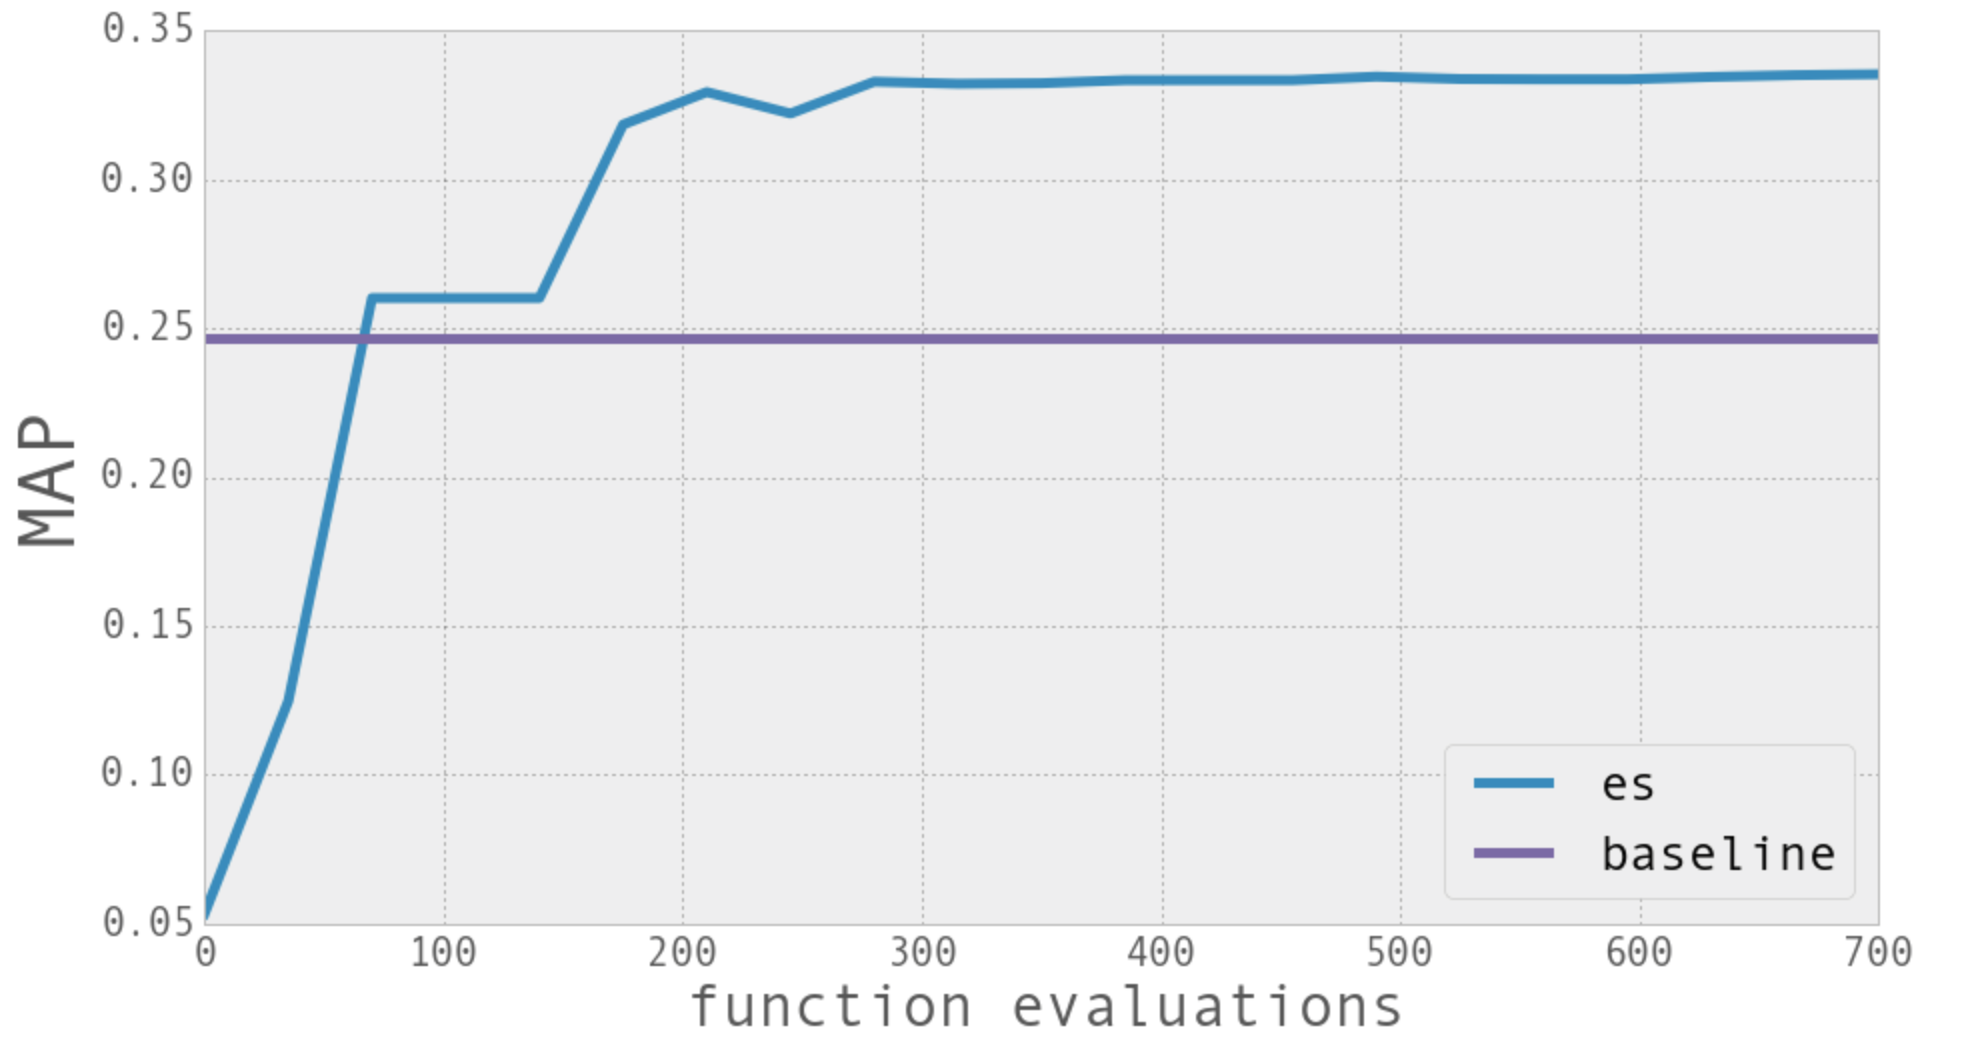
\includegraphics[width=\textwidth]{figures/es_lab3.png}
            \caption[Network2]%
            {{\small Laboratorio 3 (\textsc{baseline})}}    
            \label{fig:es_lab3}
        \end{subfigure}
        \hfill
        \begin{subfigure}[htpb]{0.475\textwidth}  
            \centering 
            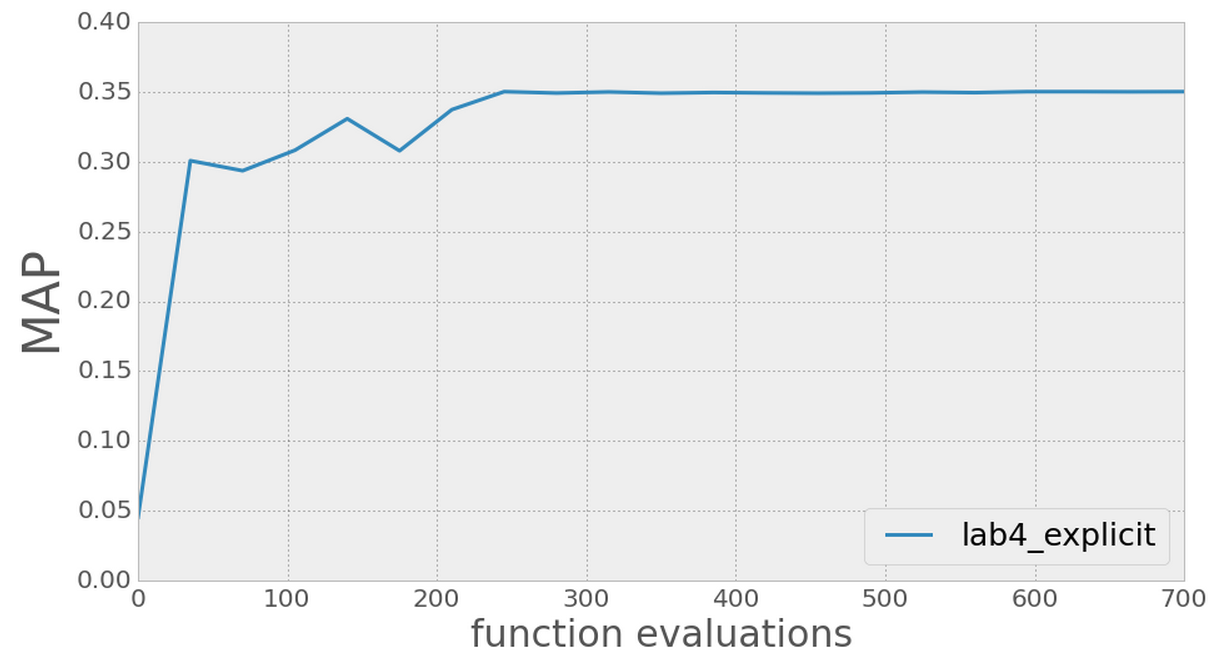
\includegraphics[width=\textwidth]{figures/es_lab4_e.png}
            \caption[]%
            {{\small Laboratorio 4 (\textsc{rf esplicito})}}    
            \label{fig:es_lab4_esp}
        \end{subfigure}
        \vskip\baselineskip
        \begin{subfigure}[htpb]{0.475\textwidth}   
            \centering 
            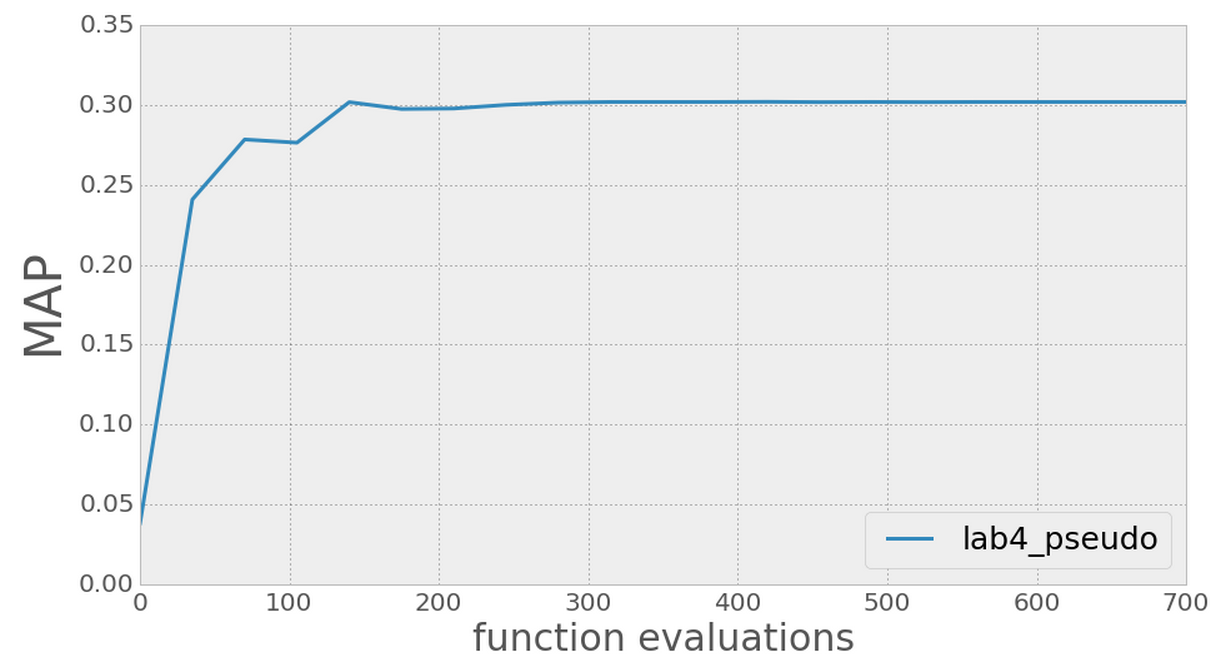
\includegraphics[width=\textwidth]{figures/es_lab4_p.png}
            \caption[]%
            {{\small Laboratorio 4 (\textsc{rf pseudo})}}    
            \label{fig:es_lab4_pse}
        \end{subfigure}
        \quad
        \begin{subfigure}[htpb]{0.475\textwidth}   
            \centering 
            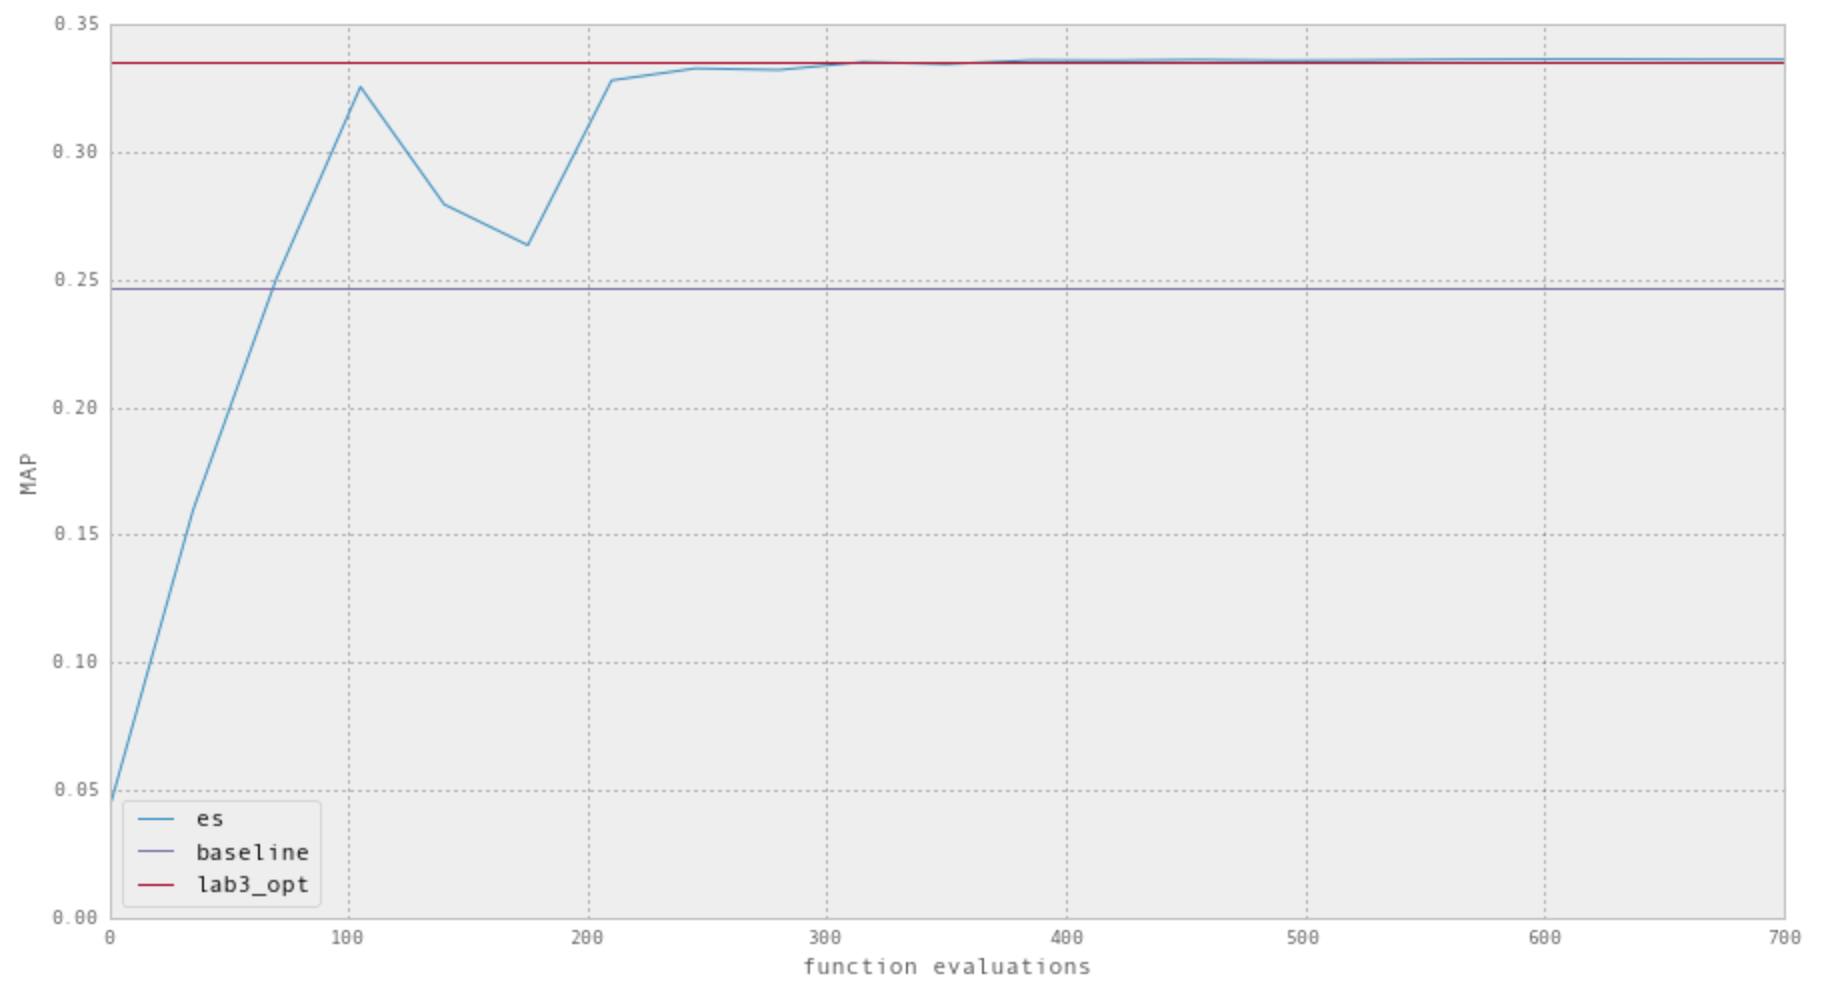
\includegraphics[width=\textwidth]{figures/es_lab5.png}
            \caption[]%
            {{\small Laboratorio 5 (\textsc{pagerank})}}    
            \label{fig:es_lab5_esp}
        \end{subfigure}
        \vskip\baselineskip
        \begin{subfigure}[htpb]{0.475\textwidth}  
            \centering 
            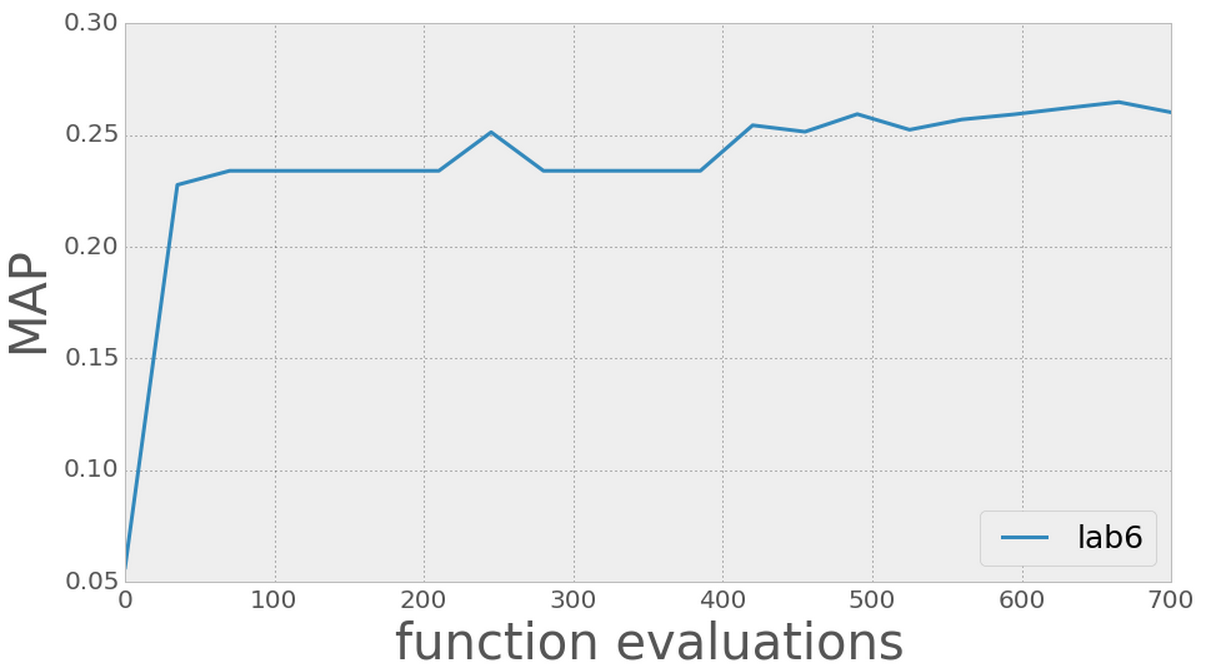
\includegraphics[width=\textwidth]{figures/es_lab6.png}
            \caption[]%
            {{\small Laboratorio 6 (\textsc{lsa})}}    
            \label{fig:es_lab6}
        \end{subfigure}
        \quad
        \begin{subfigure}[htpb]{0.475\textwidth}   
            \centering 
            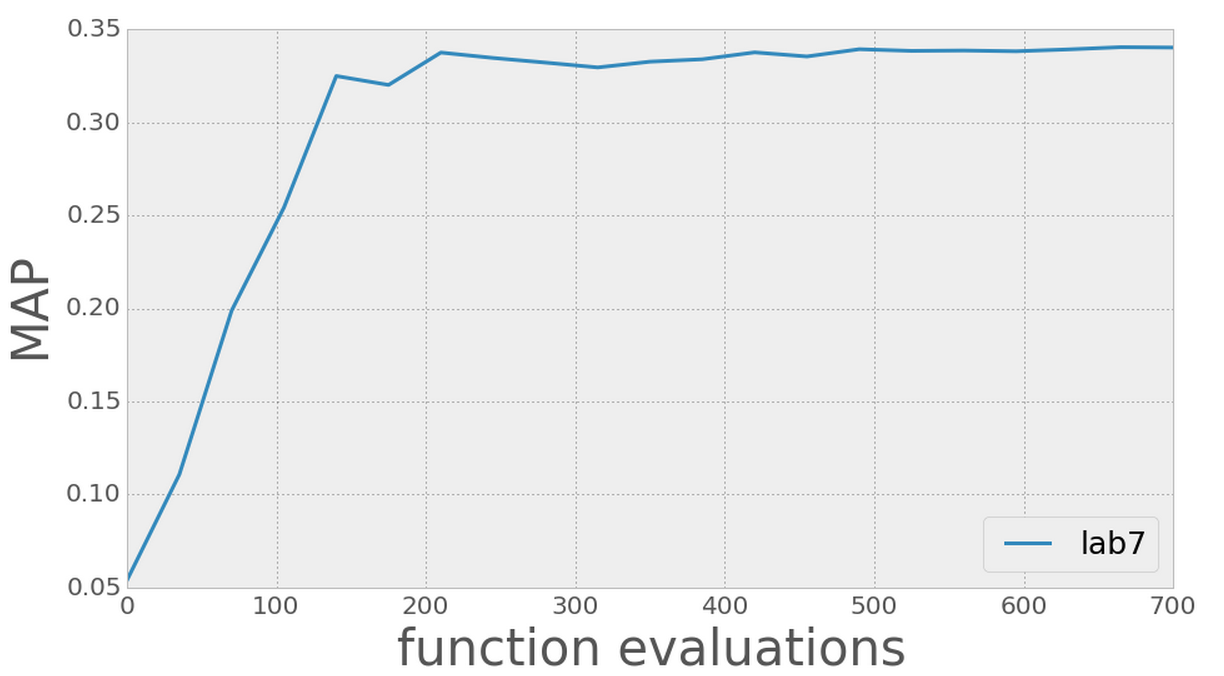
\includegraphics[width=\textwidth]{figures/es_lab7.png}
            \caption[]%
            {{\small Laboratorio 7 (\textsc{hits})}}    
            \label{fig:es_lab7}
        \end{subfigure}
        \caption[ The average and standard deviation of critical parameters ]
        {\small Valore MAP durante iterazioni dell'ES, per le funzioni di reperimento dei vari laboratori.} 
        \label{fig:es_all}
\end{figure*}
Tabella \ref{tab:es} riporta i risultati dell'ottimizzazione.
\begin{table}[htpb]

\begin{center}
\begin{tabular}{|c|c|c|}
\hline
metodo & parametri ottimizzati & MAP \\
 \hline
\textsc{baseline} & $k_1 = 0.0253, b = 0.0221$ & $0.3354$ \\
\textsc{rf} esplicito & $k_1 = 0.02065, b = 0.0$ & $0.3504$ \\
\textsc{rf} pseudo & $k_1 = 0.02065, b = 0.0$ & $0.3022$ \\
\textsc{pagerank} & $k_1 = 0.0237, b = 0.0, \alpha=0.7832$ & $0.3366$ \\
\textsc{lsa} & $k_1 = 0.0087, b = 0.0$ & $0.2648$ \\
\textsc{hits} & $k_1 = 0.0247, b = 0.0185, \alpha=1.0, \beta=0.1098, \gamma=0.0549$ & $0.3405$ \\
\hline
\end{tabular}
\end{center}
\caption{Risultati ottimizzazione con ES per le funzioni di reperimento dei vari laboratori.}
\label{tab:es}
\end{table}

Grazie all'ES si \'e ottenuto un notevole miglioramento rispetto alla prima versione dove i parametri sono stati scelti manualmente e il valore di MAP si aggirava attorno al $0.25$. Inoltre dai grafici si puo' notare come l'algoritmo di ottimizzazione sia molto robusto, dato che dopo $\sim{300}$ valutazioni \'e gia' molto vicino alla configurazione ottima. I risultati dell'ottimizzazione vengono discussi in Sezione \ref{sec:risult-sper}.

\subsection{Altri metodi}
tipo lucene
\label{sec:altri-metodi}

Se sono stati sviluppati altri metodi, descriverli qui.

